\documentclass[12pt]{article}
\usepackage{hyperref}
\usepackage{graphicx}
\usepackage{listings}
\usepackage{enumerate}
\usepackage[T1]{fontenc}
\usepackage[polish]{babel}
\usepackage[utf8]{inputenc}
\usepackage{verbatim}
\graphicspath{ {./images/} }
\def\code#1{\texttt{#1}}
\title{Kompresja danych - projekt 2}
\date{\today}
\author{Bartosz Matyjasiak}

\begin{document}
\maketitle
\tableofcontents
\pagebreak

\section{Opis problemu}
Zadanie polega na zrealizowaniu prostego kodera i dekodera wykorzystującego metodę LZ77
(dla ustalenia uwagi proszę stosować metodę w wariancie przedstawionym w materiałach
wykładowych).
Przyjmujemy następujące założenia:
\begin{enumerate}
\item Kodowane pliki mają strukturę bajtową (tzn. mogą zawierać dane z dowolnego
problemu, w którym występuje co najwyżej \textbf{256} różnych „komunikatów”).
\item Długość \textit{bufora słownika} wynosi \textbf{256} bajtów, a \textit{bufora wejściowego (look-ahead buffer)}
\textbf{15} bajtów, tzn. pojedynczy \textit{wskaźnik do słownika} ma rozmiar \textbf{2.5} bajta (\textbf{1} bajt
reprezentujący położenie kopii fragmentu znalezionej w słowniku czyli \textit{offset}, \textbf{0.5} bajta
do zakodowania \textit{długości kopii} oraz \textbf{1} bajt zawierający „komunikat” bezpośrednio po
znalezionym fragmencie).
\item Rozwiązanie ma mieć postać DWÓCH gotowych do użycia \\ funkcji/skryptów/aplikacji,
tzn. \textit{kodera} i \textit{dekodera}.
\item Koder ma dwa argumenty wejściowe, tzn. (1) nazwa wraz z rozszerzeniem
kodowanego pliku oraz (2) nazwa (wraz z dowolnie zdefiniowanym rozszerzeniem, na
przykład \textbf{.xxx}) pliku zakodowanego, który ma być zapisany w tym samym folderze,
co plik kodowany.
\item \textit{Dekoder} ma również dwa argumenty wejściowe, tzn. (1) nazwa (wraz z zastosowanym
rozszerzeniem, na przykład \textbf{.xxx}) dekodowanego pliku oraz (2) nazwa (wraz z
zadanym rozszerzeniem) pliku rozkodowanego, który ma być zapisany w tym samym
folderze, co plik dekodowany.
Zrealizowane rozwiązania powinny być przetestowane na wybranych przykładach (np. plikach
w formacie \textbf{.txt}).
\end{enumerate}
\newpage
\section{Opis rozwiązania}
Koder oraz dekoder zostały zaimplementowane w pliku \code{LZ77.py} w odpowiadających ich funkcjach \code{encode} oraz \code{decode}.
By posłuzyć się skryptem należy wybrać jeden z argumentów \code{-\--encode} lub \code{-\--decode} oraz podać nazwę pliku wejściowego oraz wynikowego.

Przykładowe użycie skryptu do zakodowania pliku \code{test.txt}:
\begin{verbatim}
  python LZ77.py --encode test.txt test.txt.lz77
\end{verbatim}

Oraz zdekodowania go:

\begin{verbatim}
  python LZ77.py --decode test.txt.lz77 test.txt.lz77.txt
\end{verbatim}

Do projektu dołączyłem też skrypt bash \code{test.sh}, 
który zakoduje przykładowe pliki w folderze \textit{input}
i zapisze jest w folderze \textit{lz77}, a następnie odkoduje je
i zapisze w folderze \textit{decoded}

\subsection{Pseudokod kodowania}
\begin{verbatim}
Dopóki w buforze wejściowym są wartości wykonuj:
  1. Wyszukaj w buforze słownikowym + buforze wejściowym najdłuższy
    ciąg wartości zaczynający się od początku bufora wejściowego,
    ciąg ten nie może mieć długość bufora wejściowego.
  2. Zapisujemy wynikową trójke (offset, characters_matching, lastchar) 
    gdzie offset jest indeksem względem pozycji startu bufora wejściowego, 
    characters_matching jest długością znalezionego ciągu wartości
    oraz lastchar jest następną wartością w buforze wejściowym po znalezionym ciągu wartości.
  3. Przesuń obydwa bufory o characters_matching+1.
\end{verbatim}
\subsection{Pseudokod dekodowania}
\begin{verbatim}
Wypełnij bufor słownikowy wartościami początkowymi
Odkoduj z pliku wszystkie trójki (offset, characters_matching, lastchar)
Dla każdej z nich wykonuj:
  Dopóki characters_matching > 0 wykonuj: 
    Skopiuj z bufora wartość z pozycji offset od końca na koniec bufora
    Zapisz ostatnią wartość z bufora jako część wyniku
    Jeżeli bufor jest większy od maksymalnego rozmiaru bufora:
      Przesuń wartości w buforze o jedną pozycje w lewo
      Usuń wartość końcową z bufora
    Zmniejsz wartość characters_matching o jeden
  
  Skopiuj wartość lastchar na koniec bufora
  Zapisz ostatnią wartość z bufora jako część wyniku
  Jeżeli bufor jest większy od maksymalnego rozmiaru bufora:
    Przesuń wartości w buforze o jedną pozycje w lewo
    Zsuń wartość końcową z bufora
\end{verbatim}

\section{Wyniki}\label{results}
\subsection{Analiza kodowania plików tekstowych}
Do przetestowania kodera użyłem dwóch tekstów:
\begin{itemize}
  \item Lokomotywa - Julian Tuwin
  \item Inwokacja - Pan Tadeusz - Adam Mickiewicz
\end{itemize}
Po uruchomieniu skryptu otrzymałem wyniki widoczne w tabelach \ref{text:1} oraz \ref{text:2}.
\begin{table}[ht!]
  \centering
  \begin{tabular}{|c|c|}
    \hline
    \multicolumn{2}{|c|}{Lokomotywa - Julian Tuwin} \\
    \hline
    \hline
    stopień kompresji & 1,309\\
    procent kompresji & 23,60\%\\
    średnia bitowa & 6,112 \\
    \hline
  \end{tabular}
  \caption{Wyniki zakodowania tekstu Lokomotywy Juliana Tuwima}
  \label{text:1}
\end{table}
\begin{table}[ht!]
  \centering
  \begin{tabular}{|c|c|}
    \hline
    \multicolumn{2}{|c|}{Inwokacja - Pan Tadeusz - Adam Mickiewicz} \\
    \hline
    \hline
    stopień kompresji & 1,160\\
    procent kompresji & 13,82\%\\
    średnia bitowa & 6,894 \\
    \hline
  \end{tabular}
  \caption{Wyniki zakodowania tekstu Inwokacji Pana Tadeusza Adama Mickiewicza}
  \label{text:2}
\end{table}

Kodowanie lz77 sprawdziło się w kompresji plików tekstowych.
W obydwu plikach średnia bitowa jest mniejsza od 8, a całe pliki zmniejszyły się o ok. 24\% oraz ok. 14\%.
Skompresowany tekst wiersza Juliana Tuwima - Lokomotywa wypadł dużo lepiej. Bardzo możliwe z przyczyny iż wiersz ten zawiera bardzo dużo rymów i powtarzających się wyrazów.
Dzięki temu koder może zaoszczędzić jeszcze więcej miejsca.

\subsection{Analiza kodowania plików audio}
Do przetestowania kodera użyłem dwóch plików audio:
\begin{itemize}
  \item icing.wav
  \item song.wav
\end{itemize}
Po uruchomieniu skryptu otrzymałem wyniki widoczne w tabelach \ref{audio:1} oraz \ref{audio:2}.
\begin{table}[ht!]
  \centering
  \begin{tabular}{|c|c|}
    \hline
    \multicolumn{2}{|c|}{icing.wav} \\
    \hline
    \hline
    stopień kompresji & 0,761\\
    procent kompresji & -31,32\%\\
    średnia bitowa & 10,506 \\
    \hline
  \end{tabular}
  \caption{Wyniki zakodowania pliku audio icing.wav}
  \label{audio:1}
\end{table}
\begin{table}[ht!]
  \centering
  \begin{tabular}{|c|c|}
    \hline
    \multicolumn{2}{|c|}{song.wav} \\
    \hline
    \hline
    stopień kompresji & 0,762\\
    procent kompresji & -31,31\%\\
    średnia bitowa & 10,505 \\
    \hline
  \end{tabular}
  \caption{Wyniki zakodowania pliku audio song.wav}
  \label{audio:2}
\end{table}

W przypadku plików audio koder nie jest najlepszym wyborem.
Obydwa pliki zwiększyły swój rozmiar o około 30\%. 


\subsection{Analiza kodowania plików graficznych}
Do przetestowania kodera użyłem trzech obrazów:
\begin{figure}[!htb]
  \minipage{.32\textwidth}
    
\includegraphics[width=\linewidth]{paski}
    \caption{img1.bmp}
  \endminipage\hfill
  \minipage{.32\textwidth}
    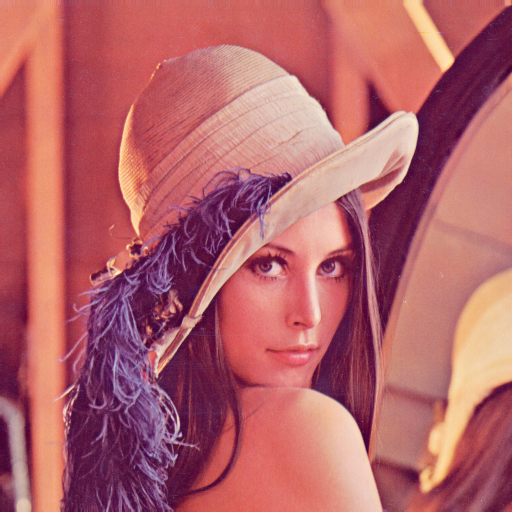
\includegraphics[width=\linewidth]{lena}
    \caption{lena.png}
  \endminipage\hfill
  \minipage{.32\textwidth}
    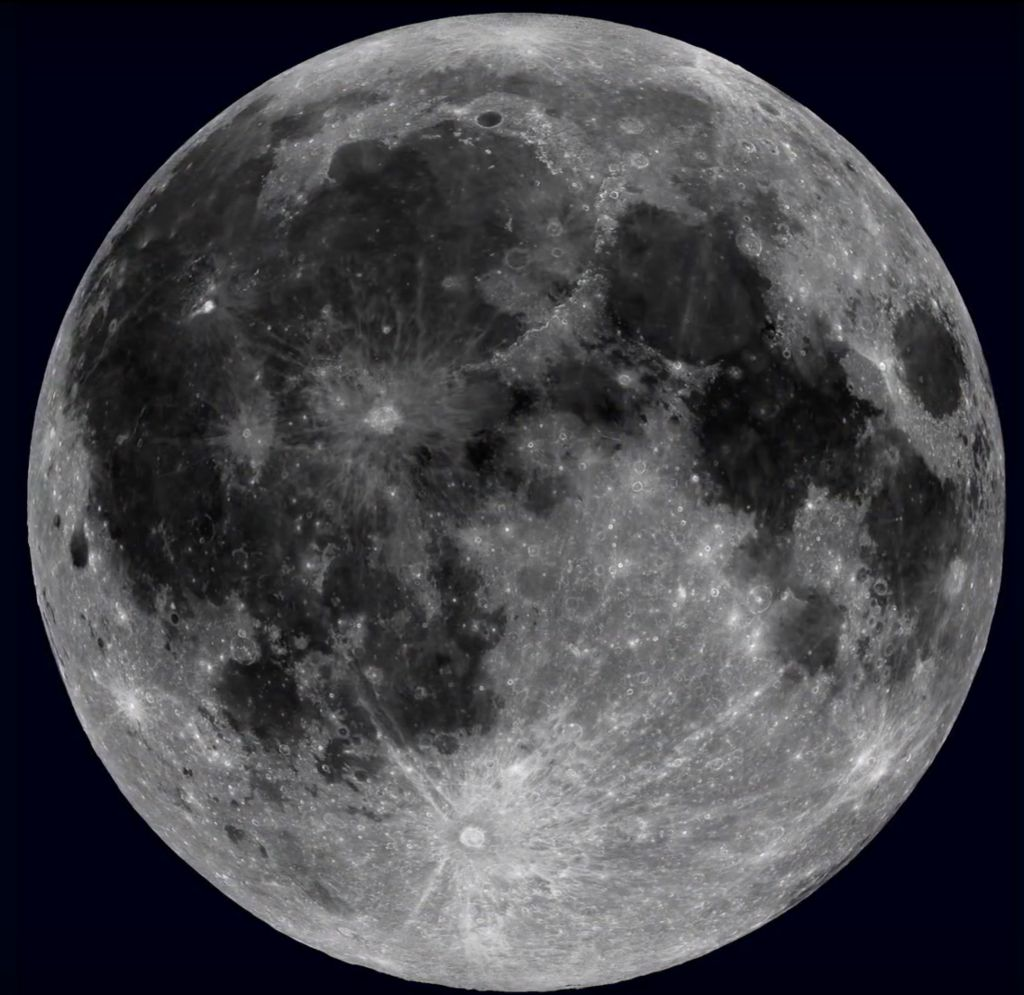
\includegraphics[width=\linewidth]{moon}
    \caption{moon.jpg}
  \endminipage
\end{figure}
Po uruchomieniu skryptu otrzymałem wyniki widoczne w tabelach \ref{image:1}, \ref{image:2} oraz \ref{image:3}.
\begin{table}[ht!]
  \centering
  \begin{tabular}{|c|c|}
    \hline
    \multicolumn{2}{|c|}{img1.bmp} \\
    \hline
    \hline
    stopień kompresji & 5,442\\
    procent kompresji & 81,63\%\\
    średnia bitowa & 1,470 \\
    \hline
  \end{tabular}
  \caption{Wyniki zakodowania pliku img1.bmp}
  \label{image:1}
\end{table}
\begin{table}[ht!]
  \centering
  \begin{tabular}{|c|c|}
    \hline
    \multicolumn{2}{|c|}{lena.png} \\
    \hline
    \hline
    stopień kompresji & 0,657\\
    procent kompresji & -52,18\%\\
    średnia bitowa & 12,174 \\
    \hline
  \end{tabular}
  \caption{Wyniki zakodowania pliku lena.png}
  \label{image:2}
\end{table}
\begin{table}[ht!]
  \centering
  \begin{tabular}{|c|c|}
    \hline
    \multicolumn{2}{|c|}{moon.jpg} \\
    \hline
    \hline
    stopień kompresji & 0,669\\
    procent kompresji & -49,52\%\\
    średnia bitowa & 11,961 \\
    \hline
  \end{tabular}
  \caption{Wyniki zakodowania pliku moon.jpg}
  \label{image:3}
\end{table}

Dla obrazów \textit{lena.png} oraz \textit{moon.jpg} wyniki kompresji są niezadowalające.
Pliki tych obrazów zwiekszyły się o około 50\%. 
Ciekawym przypadkiem jest obraz \textit{img.bmp}, który zmniejszył się aż o 81\%.
Jednak takie obrazy rzadko są spotykane w codziennym użytku.

\section{Podsumowanie}

Koder LZ77 najlepiej nadaje się do kodowania tesktu oraz obrazów z dużą powtarzalnością kolorów pikseli.
Nie nadaje się natomiast do kodowania plików audio czy też obrazów o dużej ilości szczegółów i kolorów jak portrety i krajobrazy.

\end{document}